% FastMACE preprint draft, arXiv style (11 November 2026).
% Build: latexmk -pdf main.tex   (pdflatex + bibtex)
% Every number in this file comes from a record in the repository; paper/README.md lists the sources
% and the open items (marked TODO below).
\documentclass[11pt]{article}

\usepackage[utf8]{inputenc}
\usepackage[T1]{fontenc}
\usepackage{lmodern}
\usepackage[a4paper,margin=2.6cm]{geometry}
\usepackage{amsmath,amssymb}
\usepackage{booktabs}
\usepackage{array}
\usepackage{tabularx}
\usepackage{graphicx}
\usepackage{xcolor}
\usepackage{caption}
\usepackage[numbers,sort&compress]{natbib}
\usepackage{tikz}
\usetikzlibrary{arrows.meta,positioning}
\usepackage[colorlinks=true,linkcolor=blue!50!black,citecolor=blue!50!black,urlcolor=blue!50!black]{hyperref}

\captionsetup{font=small,labelfont=bf}
\setlength{\parskip}{0.45em}
\setlength{\parindent}{0pt}
\newcommand{\angstrom}{\text{\AA}}
\newcommand{\us}{\,\ensuremath{\mu}s}
\newcommand{\ms}{\,ms}
\newcommand{\sw}[1]{\texttt{#1}}
\newcolumntype{Y}{>{\raggedright\arraybackslash}X}

\title{\textbf{FastMACE: Efficient GPU Inference and Molecular\\ Dynamics for Pretrained MACE Potentials}}

% TODO (owner): confirm the author list, affiliation and contact.
\author{Fabian Zwingel\\[0.3em]
\small University of Bayreuth, Germany}

\date{Draft of 11 November 2026}

\begin{document}
\maketitle

\begin{abstract}
\noindent
MACE potentials are accurate, but a general implementation evaluates them far below what a GPU can deliver:
each layer runs as separate kernels, every neighbour pair carries large intermediate tensors, and the molecular
dynamics loop crosses between host and device at every step. FastMACE runs \emph{unchanged pretrained
checkpoints} faster by reorganising the computation. It uses the frozen parameters to move linear work out of the
neighbour loops, replaces the radial networks with certified piecewise-polynomial tables, streams the second
interaction and its derivative without storing per-edge weights, and executes complete MD steps on the GPU as
captured CUDA graphs. A tiled evaluator with a dependency-driven schedule bounds memory for large systems.
For the OMAT-0 medium model on 5{,}000 atoms of SrTiO$_3$, recorded Langevin steps take 3.4\ms{} on an NVIDIA H200
and 6.2\ms{} on an A100, and 180 million atoms have been evaluated on a 20\,GB GPU. No retraining, distillation
or change of time step is involved. Every change is classified as an algebraic identity, a rounding change or a
sampled approximation, and is accepted only if forces and stresses stay within three times the float32
round-off of the reference implementation. We report the mechanisms, the measurements behind each, the origin of
each idea, and what remains unmeasured.
\end{abstract}

\noindent\textbf{Keywords:} machine-learned interatomic potentials, MACE, equivariant neural networks,
GPU kernels, molecular dynamics, tensor cores

\section{Introduction}

A molecular dynamics (MD) simulation evaluates the same trained potential at every step, with fixed parameters
and slowly changing geometry. A general neural-network implementation does not use that structure. For MACE
\cite{batatia2022mace}, a force call expands radial weights for every neighbour pair, forms tensor products edge
by edge, keeps the results for automatic differentiation, and returns to a host-side integrator and neighbour
list before the next step.

FastMACE is a library that runs pretrained MACE checkpoints on NVIDIA GPUs with these costs removed where the
mathematics allows it. Its unit of optimisation is the complete energy, force and MD-step calculation, not a
single layer. The work falls into four groups:
\begin{itemize}\setlength{\itemsep}{0.1em}
\item \textbf{Algebraic rewrites} that use frozen parameters and linearity (Section~\ref{sec:rewrites}).
\item \textbf{Radial tables}: the radial networks become piecewise polynomials with a setup-time certificate
      (Section~\ref{sec:tables}).
\item \textbf{Streaming kernels} for the second interaction and its derivative, and tensor-core arithmetic for
      the dense products (Sections~\ref{sec:stream} and~\ref{sec:gemm}).
\item \textbf{Execution schedules}: a GPU-resident MD engine and a tiled evaluator for large systems
      (Sections~\ref{sec:engine} and~\ref{sec:tiled}).
\end{itemize}

The paper describes these mechanisms for one concrete case, the OMAT-0 medium model in float32, and reports the
measurements on which each was adopted. Three limits of the evidence should be stated at the outset. The step
times come from separate adoption studies on different dates, not from one benchmark of a single revision. The
comparisons with other engines were made with earlier versions of FastMACE. And the numerical checks are sampled
tests on specific structures, not bounds. Section~\ref{sec:limits} lists what a full evaluation still needs.

Several of the mechanisms were first proposed elsewhere, in the literature, in other inference engines, or in
research reports produced by large language models at the author's request. Section~\ref{sec:origins} records
the origin of each.

\section{The calculation being accelerated}
\label{sec:background}

\paragraph{Model.}
MACE \cite{batatia2022mace} builds on the atomic cluster expansion \cite{drautz2019ace} and equivariant message
passing \cite{batzner2022nequip,geiger2022e3nn}. For positions $R$, cell $H$ and species $z$ the energy is
\begin{equation}
E(R,H,z) \;=\; \sum_i E^{0}_{z_i} \;+\; \sum_i \varepsilon_i(R,H,z) \;+\; E_{\text{pair}}(R,H,z),
\qquad F_i = -\frac{\partial E}{\partial R_i},
\end{equation}
where $\varepsilon_i$ is the learned site energy and $E_{\text{pair}}$ a short-range repulsion. Stress follows
from the strain derivative.

For a directed edge from sender $j$ to receiver $i$ let $r_{ij}$ be its length and $Y_b(\hat r_{ij})$ its real
spherical harmonics. An interaction forms the message
\begin{equation}
m^{(p)}_{i,o,c} \;=\; \sum_{j \in \mathcal N(i)} w_{p,c}(r_{ij})
\sum_{a,b} C^{(p)}_{oab}\; x_{j,a,c}\; Y_b(\hat r_{ij}),
\label{eq:message}
\end{equation}
with channel $c$, coupling path $p$, input and output components $a$ and $o$, Clebsch--Gordan coefficients $C$,
and radial weights $w$ produced by a small network of the distance (and of the two species). A symmetric
contraction then forms polynomial combinations of the message at each atom, equivariant linear maps mix channels,
and readouts give $\varepsilon_i$.

\paragraph{The example model.}
All details below refer to OMAT-0 medium, a two-interaction MACE foundation model
\cite{batatia2023foundation} trained on the OMat24 data \cite{barroso2024omat24}. It has 128 channels, harmonics
up to degree 3 (16 components), a 6\,\angstrom{} cutoff, and symmetric contractions up to third order. The second
interaction receives 512 features per atom and has 10 paths, so each edge carries $10\times128 = 1{,}280$ radial
weights. Its final readout contains a nonlinear layer.

\paragraph{Where a general implementation spends its work.}
The benchmark used throughout is SrTiO$_3$, $10\times10\times10$ cells, 5{,}000 atoms and about 370{,}000
directed edges (74 per atom). Storing the second interaction's weights alone takes
$370{,}000 \times 1{,}280 \times 4$ bytes $\approx 1.9$\,GB per force call, and their gradient the same again.
The standard MD loop adds a host-side integrator and a neighbour search at every step, with two transfers between
host and device.

\section{Design}
\label{sec:design}

FastMACE keeps MACE's own PyTorch modules and rewrites a private copy of the model. This differs from engines
that convert the checkpoint into their own representation \cite{fu2026symmetrixxl}. Figure~\ref{fig:overview}
shows the structure.

\begin{figure}[t]
\centering
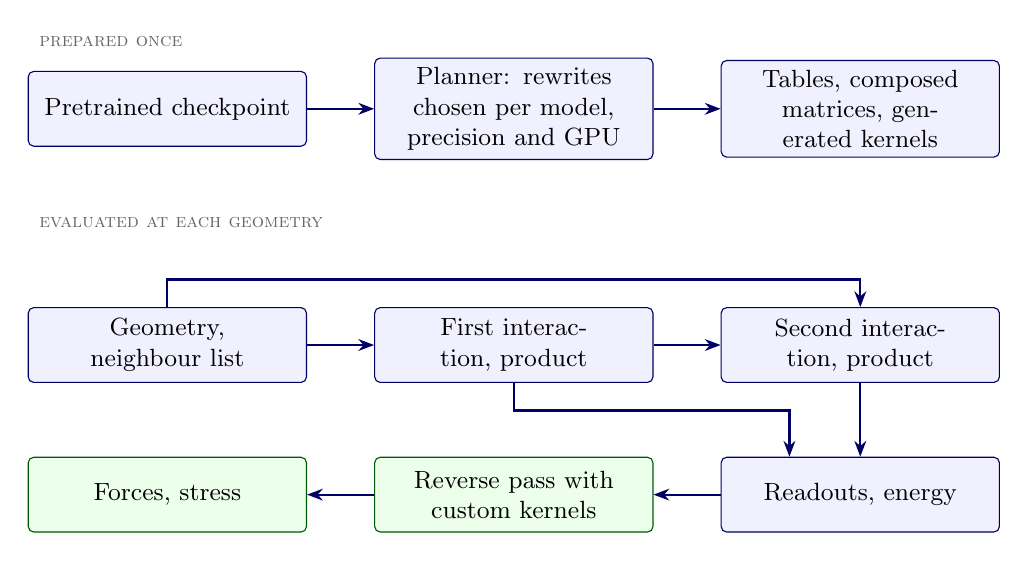
\begin{tikzpicture}[
  box/.style={draw=blue!40!black, fill=blue!6, rounded corners=2pt, minimum height=0.95cm,
              text width=3.3cm, align=center, font=\small},
  outbox/.style={box, fill=green!8, draw=green!35!black},
  lab/.style={font=\scriptsize\scshape, text=black!60},
  arr/.style={-{Stealth[length=2mm]}, thick, draw=blue!40!black}]
\node[lab, anchor=west] at (-1.75,1.75) {prepared once};
\node[box] (ck) at (0,0.9) {Pretrained checkpoint};
\node[box] (pl) at (4.4,0.9) {Planner: rewrites chosen per model, precision and GPU};
\node[box] (tb) at (8.8,0.9) {Tables, composed matrices, generated kernels};
\draw[arr] (ck) -- (pl); \draw[arr] (pl) -- (tb);
\node[lab, anchor=west] at (-1.75,-0.55) {evaluated at each geometry};
\node[box] (ge) at (0,-2.1) {Geometry, neighbour list};
\node[box] (i1) at (4.4,-2.1) {First interaction, product};
\node[box] (i2) at (8.8,-2.1) {Second interaction, product};
\node[outbox] (fo) at (0,-4.0) {Forces, stress};
\node[outbox] (rv) at (4.4,-4.0) {Reverse pass with custom kernels};
\node[box] (ro) at (8.8,-4.0) {Readouts, energy};
\draw[arr] (ge) -- (i1); \draw[arr] (i1) -- (i2); \draw[arr] (i2) -- (ro);
\draw[arr] (ro) -- (rv); \draw[arr] (rv) -- (fo);
\draw[arr] (ge.north) -- ++(0,0.35) -| (i2.north);
\draw[arr] (i1.south) -- ++(0,-0.35) -| ([xshift=-0.9cm]ro.north);
\end{tikzpicture}
\caption{Structure of FastMACE. Preparation is allowed to be expensive because its products are reused. The
repeated calculation is captured in CUDA graphs. A tiled evaluator (Section~\ref{sec:tiled}) reuses the same
rewritten modules with a different storage schedule.}
\label{fig:overview}
\end{figure}

\paragraph{Rewrites and their classes.}
Each change is a \emph{rewrite} that the planner turns on for a model, precision and GPU. Every rewrite belongs
to one of three classes, which the paper keeps apart:
\begin{itemize}\setlength{\itemsep}{0.1em}
\item \textbf{Identity in real arithmetic}: composing linear maps, moving a linear map through a sum. Only
      rounding changes.
\item \textbf{Rounding change}: a different summation order or a tensor-core decomposition of a product.
\item \textbf{Sampled approximation}: radial tables and packed coefficients, accepted by a numerical check at
      setup.
\end{itemize}
Some rewrites assume frozen parameters and provide no training gradients.

\paragraph{How defaults are chosen.}
A rewrite becomes a default for a GPU family only after a paired timing in one process, with alternating blocks
and both build orders, shows it faster in both, and after the accuracy gate of Section~\ref{sec:validation}
passes. The noise floor of this comparison was measured at 0.2\,\% to 1.1\,\% depending on the machine. A rewrite
that only removes work is enabled everywhere after one such test. Defaults therefore differ between GPUs
(Table~\ref{tab:routes}).

\paragraph{Software.}
The fast path is a PyTorch computation with specialised operators. PyTorch's compiler
\cite{ansel2024pytorch2} fuses elementwise regions; Triton \cite{tillet2019triton}, run-time compiled CUDA,
CUTLASS \cite{cutlass} and cuEquivariance \cite{cuequivariance} implement individual operations; automatic
differentiation connects custom reverse kernels to the rest.

\section{Rewrites that use frozen parameters}
\label{sec:rewrites}

\subsection{Aggregate before projecting in the first interaction}

In the first interaction the sender features depend only on the species. Together with the fact that the last
layer of the radial network is linear, this allows the projection onto the 128 channels to move outside the
neighbour sum. With $a_k(r)$ the hidden radial features (64 per species pair, cutoff included),
\begin{align}
S_{i,z,b,k} &= \sum_{j\in\mathcal N(i),\; z_j = z} a_k(r_{ij};z_i,z)\; Y_b(\hat r_{ij}), \\
m_{i,b,c}   &= \sum_{z,k} W^{(b)}_{z,c,k}\; S_{i,z,b,k},
\end{align}
where $W$ combines the frozen radial matrix, the species features and the path normalisation. The edge loop then
accumulates $16\times64$ numbers per receiver and sender species, and the projection is a dense product per atom.
This is the density trick of the atomic cluster expansion \cite{drautz2019ace} applied to MACE's first layer.
Later interactions have environment-dependent sender features and cannot use it.

The implementation evaluates the radial table inside the edge walk and never writes an edge-by-feature array. Its
reverse recomputes values and slopes, contracts the local adjoint into a distance derivative at once, and
discards it.

\subsection{Composing adjacent linear maps}

With frozen parameters, adjacent linear maps can be multiplied during preparation. FastMACE folds the linear map
after the first product into its three consumers (the second interaction's input projection, its
species-dependent skip map and the first readout), composes the first interaction's projection with its linear
map and species skip, and composes the map into the final readout with the preceding product, so that the readout
tail runs at 16 instead of 128 channels. Nonlinearities stay in place.

\subsection{A generated symmetric contraction}

The first symmetric contraction is a fixed polynomial for a given checkpoint: 16 angular inputs and four outputs
per channel in OMAT-0 medium. FastMACE generates a straight-line program for it from the contraction's
descriptor, with repeated products shared, together with its reverse. A factored variant evaluates the same
polynomial through shared pair products in a basis of 13 scalar invariants and 16 vector covariants, with the
species-dependent weights transformed at setup. The division by the neighbour density that follows the first
interaction is fused into the same kernel. On the H200 the four kernels this replaces took 179.5\us{} per force
call and the generated pair takes 82.4\us{}.

\section{Radial functions as certified tables}
\label{sec:tables}

A frozen radial network is a function of one variable per species pair. FastMACE evaluates it in float64 at setup
and stores a piecewise polynomial, which removes the radial embedding, the hidden layers and the cutoff from the
force loop. Tabulating an embedding network is established practice in other potentials
\cite{lu2022dpcompress}; the specific forms here follow from what each interaction consumes.

\paragraph{First interaction.}
It needs the hidden features $a_k(r)$. They are stored as Chebyshev series \cite{trefethen2013atap} of degree 5
on adaptively chosen pieces, together with the cutoff and density terms.

\paragraph{Second interaction.}
It reads the 1{,}280 weights directly from cubic Hermite splines on piecewise-uniform knots, evaluated in the
power basis,
\begin{equation}
w(r) \approx c_0 + t\,(c_1 + t\,(c_2 + t\,c_3)), \qquad t = (r-r_k)/h_k .
\end{equation}
This removes the hidden-to-weight matrix product from every force call. Reading the weights from splines in a
receiver-major kernel follows Symmetrix-XL \cite{fu2026symmetrixxl}; the spline construction and its check are
our own.

\paragraph{The certificate.}
A table is accepted at setup only if, on uniform and random samples of the distance, the error of the float32
table against the float64 network is no larger than the error of the float32 network itself, for values and for
first derivatives. This is a sampled test, not a bound for every distance.

\paragraph{A packed table for the forward pass.}
On the forward pass the table is the dominant stream of bytes. An optional packed form stores eight bytes per
weight instead of sixteen: the cubic is replaced by a quadratic in a centred coordinate, with three fixed-point
coefficients and a shared exponent. The reverse pass keeps the float32 cubic. \emph{The forces are then not the
exact gradient of the reported energy.} Both remain within the acceptance rule of
Section~\ref{sec:validation}, but the two are no longer consistent to round-off, and we have no energy-drift
record for this path yet (Section~\ref{sec:limits}).

\section{Streaming the second interaction}
\label{sec:stream}

\paragraph{Forward.}
Work is assigned to receiver-and-channel pairs. One thread walks a receiver's edges, evaluates the radial
weights, contracts sender features with the harmonics, and accumulates the 40 output components of its channel
in registers. The result is written once, already in the block layout of the following linear maps. Neither the
edge messages nor the radial weights are materialised. Edges are staged in tiles of 32 in shared memory, and each
receiver's edges are sorted by length so that neighbouring receivers read the same table pieces.

The kernels descend from the receiver-streaming convolution of Fuchs \cite{fuchs2026oeqpr223} in
OpenEquivariance \cite{bharadwaj2025oeq}, which adapts the schedule of Sobek \cite{chorosajev2026sobek}; the
adapted files keep the upstream licence.

\paragraph{Reverse without stored weights.}
For one edge, path and channel let $g_o$ be the adjoint of the receiver's message. With
\begin{equation}
u_a = \sum_{o,b} C_{oab}\, g_o\, Y_b, \qquad
v_b = \sum_{o,a} C_{oab}\, g_o\, x_a, \qquad
q = \sum_a x_a u_a ,
\end{equation}
the three adjoints are
\begin{equation}
\bar x_a \mathrel{+}= w\,u_a, \qquad \bar Y_b \mathrel{+}= w\,v_b, \qquad \bar r \mathrel{+}= w'\,q .
\end{equation}
The kernel rebuilds $w$ and its slope $w'$ from the table, so the edge-weight gradient tensor and the dense
projection through it never exist. The receiver's adjoint row is copied to shared memory once per run of edges.

\paragraph{What limits these kernels.}
Table~\ref{tab:profile} shows that the second interaction is about 53\,\% of the kernel time of a force call. On
the A100 both of its kernels are bound by the fused multiply-add units (84--85\,\% busy); on the H200 they are
bound by instruction issue. This shapes what further changes can gain (Section~\ref{sec:limits}).

\begin{table}[t]
\centering
\small
\begin{tabular}{lrrrr}
\toprule
 & \multicolumn{2}{c}{H200} & \multicolumn{2}{c}{A100-SXM4-80GB} \\
Component & $\mu$s & share & $\mu$s & share \\
\midrule
Second interaction, reverse  & 1{,}089 & 33\,\% & 2{,}256 & 35\,\% \\
Second interaction, forward  &   629 & 19\,\% & 1{,}255 & 19\,\% \\
Dense products (tensor cores) &  609 & 19\,\% & 1{,}069 & 16\,\% \\
First interaction, forward and reverse & 323 & 10\,\% & 844 & 13\,\% \\
Symmetric contractions       &   192 &  6\,\% &   402 &  6\,\% \\
Other (geometry, elementwise, reductions) & 416 & 13\,\% & 686 & 11\,\% \\
\midrule
Total                        & 3{,}258 &  & 6{,}512 & \\
\bottomrule
\end{tabular}
\caption{Kernel time of one force call (OMAT-0 medium, SrTiO$_3$, 5{,}000 atoms), from a hardware-counter
profile of 9 November 2026. The profile predates the generated contraction on the H200 and the hybrid product on
the A100.}
\label{tab:profile}
\end{table}

\section{Dense products on tensor cores}
\label{sec:gemm}

After the edge work, dense per-atom products are the next largest cost. Tensor cores multiply at reduced
precision, so a float32 operand is split into a high part and a residual, and three reduced-precision products
recover the high--high term and the two cross terms \cite{ootomo2022tf32}. The residual--residual term is
dropped. FastMACE uses the CUTLASS kernel for this \cite{cutlass}, with the division by the density and the
species selection fused into its output stage.

On the A100 a hybrid variant computes the high--high term in TF32 and packs both cross terms into one half-precision
product,
\begin{equation}
AB \;\approx\; A_h B_h \;+\; 2^{-11}\,\bigl[\,A_h \;\; A_l'\,\bigr]\!\begin{bmatrix} B_l' \\ B_h \end{bmatrix},
\qquad A_l' = 2^{11}(A - A_h),
\end{equation}
with float32 accumulation. This takes two tensor-core instructions per step instead of three. Its error is at or
below that of the three-product kernel on every tested shape, and it ran at 0.87 of that kernel's time summed
over nine representative shapes. The operands must stay below 32{,}752 in magnitude; the recorded operands of
this model are far below, but there is no run-time guard.

\begin{table}[t]
\centering
\small
\begin{tabular}{lll}
\toprule
GPU & Dense products & First symmetric contraction \\
\midrule
H200            & CUTLASS, three TF32 products     & generated \\
A100-SXM4-80GB  & CUTLASS, hybrid TF32 / FP16      & generated, factored \\
RTX 4000 Ada    & Triton, three TF32 products      & generated, factored \\
RTX 5060 Ti     & float32                          & cuEquivariance \\
\bottomrule
\end{tabular}
\caption{Routes chosen by measurement for OMAT-0 medium in float32. The differences reflect which unit limits
each GPU.}
\label{tab:routes}
\end{table}

\section{Executing complete MD steps}
\label{sec:engine}

Positions, velocities and forces stay on the GPU. A step replays two captured CUDA graphs
\cite{cudagraphs}: the first integrates, checks displacements and compacts the neighbour candidates to the
cutoff; the second evaluates forces and completes the integration. Graphs are captured for padded edge counts,
and padding contributes exactly zero.

\paragraph{Pipelining.}
The engine launches the force graph before the host has read the flags of the first graph. If the edge count has
outgrown the capacity, or the neighbour list has expired, the engine restores the saved mid-step state and
repeats the force stage with the same random numbers. The profiled runs had no repeated steps. The measured gaps
between kernels were 63\us{} in a 3.24\ms{} force graph on the H200.

\paragraph{Neighbour list.}
The list holds pairs within the cutoff plus a skin \cite{verlet1967} and is rebuilt on the GPU. In fixed-cell
runs the rebuild starts early, on a second stream, beside the force evaluation. For more than 10{,}000 atoms a
cell-list screen replaces the pairwise screen of tiles (Section~\ref{sec:large}). Langevin noise is drawn in
batches of 256 steps on a background thread.

None of this changes the time step, skips a force evaluation or reuses stale features.

\section{Tiled evaluation for large systems}
\label{sec:tiled}

The whole-system path keeps every intermediate of a force call in device memory. For larger systems FastMACE
partitions the atoms into receiver tiles; a tile owns the edges that end at its receivers and gathers the sender
halo they need. Evaluating a two-interaction model tile by tile in three sweeps, with only the inter-layer state
global, is the tiled mode of Symmetrix-XL \cite{fu2026symmetrixxl}, which we follow. The following parts are our
own.

\paragraph{Storing what the next interaction reads.}
Instead of the features $h$ after the first product, FastMACE stores $x = A h$ and $s = B_z h$, the two
quantities the second interaction reads: 512 and 128 float32 values per atom. The three sweeps are then:
\begin{enumerate}\setlength{\itemsep}{0.1em}
\item evaluate the first interaction without a tape and store $x$ and $s$;
\item evaluate the second interaction and differentiate, giving direct edge derivatives and the adjoints
      $g^x$, $g^s$;
\item recompute the first interaction and differentiate the surrogate
      $\Phi_T = \sum_{i\in T}\bigl[\varepsilon^{(1)}_i + \langle g^x_i, x_i\rangle + \langle g^s_i, s_i\rangle\bigr]$
      with the adjoints held fixed.
\end{enumerate}

\paragraph{Wavefront and row reuse.}
A row of $s$ can be overwritten by its adjoint as soon as its own tile has run, and a row of $x$ once its last
reader has run. A wavefront schedule interleaves the three sweeps along one axis of the tile grid, so that only a
band of tiles holds state at any time. The state can live on the device or in host memory.

\paragraph{Coordinates.}
In boxes larger than about 64\,\angstrom{} float32 positions lose enough precision to produce visible force
errors on a perfect crystal ($1.3\times10^{-3}$\,eV/\angstrom{} at 1{,}200\,\angstrom). Edge vectors are
therefore formed from float64 positions in a tile-local frame, which reduces that residual to
$4\times10^{-6}$\,eV/\angstrom{}.

\section{Numerical validation}
\label{sec:validation}

\paragraph{Acceptance rule.}
Production results are compared with a float64 reference. The float32 result of the reference implementation
(MACE under ASE \cite{larsen2017ase}) serves as the yardstick. For energy per atom, the largest force component
and the largest stress component, each over the tested configurations,
\begin{equation}
e_{\text{production}} \;\le\; \max\bigl(3\, e_{\text{float32}},\; f\bigr),
\end{equation}
with floors $f$ of 0.01\,meV/atom, $10^{-5}$\,eV/\angstrom{} and $10^{-7}$\,eV/\angstrom$^3$. The test
configurations are rattled and strained supercells of SrTiO$_3$, NaCl and NbCl$_5$.

\paragraph{History of the threshold.}
The factor was 2 until 7 November 2026. It was raised to 3 after one A100 configuration exceeded the limit in a
single quantity (NbCl$_5$ stress, $1.8\times10^{-7}$ against $1.2$--$1.5\times10^{-7}$\,eV/\angstrom$^3$). The
current A100 configuration passes that check at a ratio near 1.

\begin{table}[t]
\centering
\small
\begin{tabular}{llccc}
\toprule
GPU and configuration & Quantity & SrTiO$_3$ & NaCl & NbCl$_5$ \\
\midrule
H200, 9 Nov 2026            & forces & 0.85 & 0.92 & 0.96 \\
                            & stress & 0.42 & 0.78 & 1.21 \\
A100, 11 Nov 2026           & forces & 0.98 & 0.86 & 0.99 \\
                            & stress & 0.67 & 0.89 & 1.31 \\
A100 with hybrid product    & forces & 0.94 & 0.87 & 1.00 \\
                            & stress & 0.55 & 0.96 & 1.25 \\
\bottomrule
\end{tabular}
\caption{Error of the production path relative to the float32 error of the reference implementation (limit 3).
For scale, the reference's float32 force error is about $3\times10^{-5}$\,eV/\angstrom{} on SrTiO$_3$.}
\label{tab:gate}
\end{table}

\paragraph{Results.}
Table~\ref{tab:gate} gives the recorded ratios. The production path is at or below the float32 error of the
reference in forces and within 1.3 times in stress.

\paragraph{Energy conservation.}
In an NVE run of NaCl (216 atoms, 10\,ps) the energy drift per atom was $-4\times10^{-6}$\,meV/ps with the
Chebyshev tables and $9\times10^{-7}$\,meV/ps without them. This record predates the packed forward table.

\paragraph{What the check does not show.}
Passing establishes numerical agreement with the reference on those configurations. It is not a bound over all
geometries, not a guarantee for long trajectories, and says nothing new about agreement with quantum-mechanical
data. Reduced-precision storage of the tiled state (float16) fails the rule by factors of 12 to 51 and is offered
only as a capacity fallback.

\section{Performance}
\label{sec:performance}

\paragraph{Protocol.}
Unless stated otherwise: OMAT-0 medium, float32, SrTiO$_3$ with 5{,}000 atoms, Langevin dynamics at 300\,K, 1\,fs
time step, 0.5\,\angstrom{} skin. Each engine is warmed up for 200 steps and timed over six blocks of 256 steps,
synchronised at block boundaries. Integration and neighbour maintenance are included; construction, compilation
and warm-up are not. Paired numbers are the two build orders of an A/B study.

\subsection{Step times}

\begin{table}[t]
\centering
\small
\begin{tabular}{llcc}
\toprule
GPU & Date of record & ms per step & $\mu$s per atom and step \\
\midrule
H200            & 9 Nov 2026     & 3.40 / 3.37   & 0.68 \\
A100-SXM4-80GB  & 11 Nov 2026    & 6.24 / 6.23   & 1.25 \\
RTX 4000 Ada    & 10--11 Nov 2026 & 17.67 / 17.76 & 3.5 \\
RTX 5060 Ti     & 10--11 Nov 2026 & $\approx 15.4$ & 3.1 \\
\bottomrule
\end{tabular}
\caption{Recorded steady-state MD step times. Each row comes from its own adoption study and source revision;
this is not a controlled comparison of the GPUs.}
\label{tab:steps}
\end{table}

Table~\ref{tab:steps} gives the recorded times. Figure~\ref{fig:history} shows how the A100's step time fell as
defaults were adopted between 3 and 11 November 2026.

\begin{figure}[t]
\centering
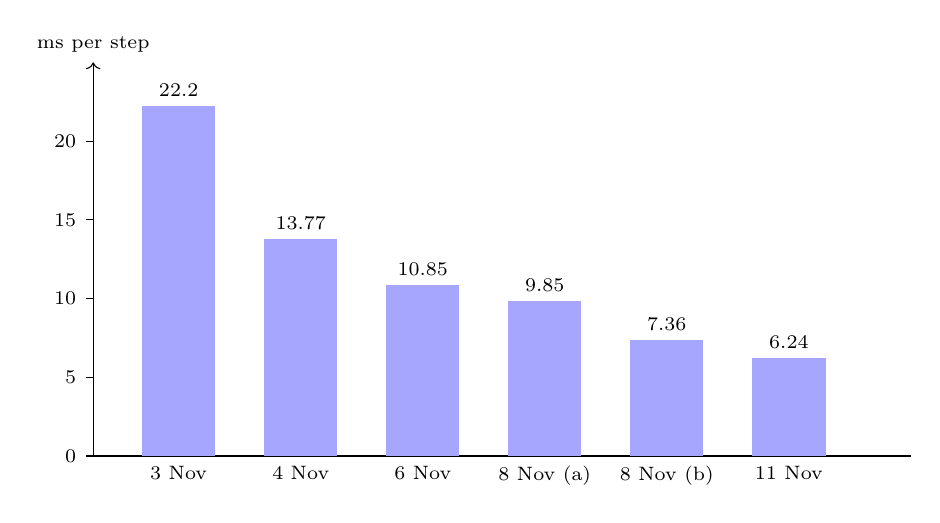
\begin{tikzpicture}[x=1.55cm,y=0.2cm]
\draw[->] (0.3,0) -- (0.3,25) node[above,font=\scriptsize] {ms per step};
\draw (0.3,0) -- (7.0,0);
\foreach \y in {0,5,10,15,20} \draw (0.3,\y) -- ++(-0.06,0) node[left,font=\scriptsize] {\y};
\foreach \i/\v/\l in {1/22.2/3 Nov,2/13.77/4 Nov,3/10.85/6 Nov,4/9.85/{8 Nov (a)},5/7.36/{8 Nov (b)},6/6.24/11 Nov}{
  \fill[blue!35] (\i-0.3,0) rectangle (\i+0.3,\v);
  \node[above,font=\scriptsize,text=black] at (\i,\v) {\v};
  \node[below,font=\scriptsize,text=black] at (\i,0) {\l};
}
\end{tikzpicture}
\caption{Recorded MD step time on the A100-SXM4-80GB for successive default configurations (SrTiO$_3$, 5{,}000
atoms). The values come from different jobs and are not paired measurements. Main changes between bars: custom
second-interaction kernels and degree-5 tables (4 Nov); staging and fused first interaction (6 Nov); spline
weights, receiver-major forward and composed first-interaction maps (8 Nov; bars a and b are the two sides of
that paired study); packed table, generated contraction and hybrid product (11 Nov).}
\label{fig:history}
\end{figure}

\subsection{Effect of individual changes}

\begin{table}[t]
\centering
\small
\renewcommand{\arraystretch}{1.15}
\begin{tabularx}{\textwidth}{Yllc}
\toprule
Change & GPU & Date & Step time ratio (two orders) \\
\midrule
Radial tables (first evidence)                  & A100 PCIe & 3 Nov  & 0.902 / 0.901 \\
Reverse rebuilds weights from the table         & A100      & 4 Nov  & 0.943 / 0.943 \\
Factored reverse                                & A100      & 4 Nov  & 0.938 / 0.940 \\
Fused first-interaction forward and reverse     & A100      & 5 Nov  & 0.966 / 0.962 \\
Spline weights, receiver-major forward, composed maps (ten switches) & A100 & 8 Nov & 0.747 / 0.747 \\
Edges sorted by length                          & H200      & 8 Nov  & 0.981 / 0.979 \\
Packed forward table                            & A100      & 9 Nov  & 0.956 / 0.955 \\
                                                & RTX 4000 Ada & 11 Nov & 0.904 / 0.903 \\
Generated symmetric contraction                 & H200      & 9 Nov  & 0.976 / 0.973 \\
                                                & A100 PCIe & 9 Nov  & 0.969 / 0.965 \\
Shared geometry sums in the forward             & A100      & 10 Nov & 0.976 / 0.981 \\
Hybrid TF32 / FP16 product                      & A100      & 11 Nov & 0.990 / 0.988 \\
\bottomrule
\end{tabularx}
\caption{Paired step-time ratios (new over old, below 1 is faster) from the studies on which each change was
adopted. The baselines differ from row to row, so the ratios do not multiply to the totals of
Figure~\ref{fig:history}.}
\label{tab:ab}
\end{table}

Table~\ref{tab:ab} lists the paired measurements behind the main mechanisms. The local kernel saving and the
whole-step saving agree where both were measured: the generated contraction saved 97\us{} of kernel time on the
H200 and 84--93\us{} per step.

\subsection{Comparison with other engines}

Table~\ref{tab:engines} collects the recorded comparisons. \emph{All of them were made with earlier versions of
FastMACE and on single dates}; they are not a synchronised benchmark, and the other engines have since moved on
as well. With that caveat: on small cells, FastMACE was 3 to 23 times faster per step than ASE with MACE's
calculator, TorchSim and the ALCHEMI Toolkit in October. On the 5{,}000-atom benchmark, Symmetrix-XL under
LAMMPS \cite{thompson2022lammps} was faster than FastMACE on 3 November (25.0 against 26.5\ms{}); three days
later FastMACE was 2.5 times faster than Symmetrix-XL 0.1.2 on the H200, and its step time has since fallen by a
further 40\,\%.

\begin{table}[t]
\centering
\small
\setlength{\tabcolsep}{4pt}
\begin{tabularx}{\textwidth}{>{\raggedright\arraybackslash}p{3.7cm}Yllc}
\toprule
 & & \multicolumn{2}{c}{Step time} & \\
\cmidrule(lr){3-4}
Engine & GPU, model, system & other engine & FastMACE & Date \\
\midrule
ASE 3.27 with MACE's calculator (cuEquivariance) & RTX 5060 Ti, MH-1, NaCl (216) / NbCl$_5$ (1{,}944) &
   41.4 / 135\ms & 3.1 / 21.3\ms & 24 Oct \\ \addlinespace[3pt]
TorchSim 0.6.2 \cite{torchsim}, best compile mode & RTX 5060 Ti, OMAT-0 medium, same systems &
   16.3 / 39.4\ms & 1.62 / 9.79\ms & 25 Oct \\ \addlinespace[3pt]
ALCHEMI Toolkit 0.2.0 \cite{alchemi} & RTX 5060 Ti, OMAT-0 medium, same systems &
   15.8 / 27.3\ms & 1.65 / 9.91\ms & 26 Oct \\ \addlinespace[3pt]
Symmetrix-XL under LAMMPS \cite{fu2026symmetrixxl} & A100 80GB PCIe, OMAT-0 medium, SrTiO$_3$ (5{,}000) &
   25.0\ms & 26.5\ms & 3 Nov \\ \addlinespace[3pt]
Symmetrix-XL 0.1.2 & H200, same model and system & 14.6\ms & 5.72\ms & 6 Nov \\
\bottomrule
\end{tabularx}
\caption{Recorded MD step times of other engines and of FastMACE on the same day and machine. FastMACE's later
times for the last two systems are in Table~\ref{tab:steps}.}
\label{tab:engines}
\end{table}

\subsection{Larger systems}
\label{sec:large}

\paragraph{Neighbour search.}
The pairwise screen of the rebuild grows with the square of the atom count. On an RTX 5060 Ti a rebuild takes
25\ms{} at 20{,}480 atoms and 2.1\,s at 214{,}375 atoms; the cell-list screen brings these to 8 and 73\ms{}
with a bit-identical list. In MD the step time ratio was 0.98 at 20{,}480 atoms and 0.96 at 40{,}000 atoms.

\paragraph{Capacity.}
Table~\ref{tab:capacity} gives the largest recorded systems. The whole-system path reaches a few hundred thousand
atoms on 16--20\,GB cards. The tiled path with the wavefront schedule and host state has evaluated 180 million
atoms on a 20\,GB card in float32. A 398-million-atom call on an 80\,GB A100 stored the state in float16 and is
therefore not a validated float32 result.

\begin{table}[t]
\centering
\small
\setlength{\tabcolsep}{4pt}
\begin{tabularx}{\textwidth}{>{\raggedright\arraybackslash}p{4.3cm}Yrr}
\toprule
Path & GPU & Atoms (SrTiO$_3$) & Per force call \\
\midrule
Whole system      & RTX 5060 Ti, 16\,GB      & 214{,}375       & -- \\
Whole system      & RTX 4000 Ada, 20\,GB     & 296{,}595       & -- \\ \addlinespace[3pt]
Tiled, device state & A100-SXM4-80GB         & 975{,}560       & 2.04\,s (2.1\us/atom) \\
Tiled, device state & RTX 5060 Ti            & 975{,}560       & 6.1--6.3\,s (6.3\us/atom) \\ \addlinespace[3pt]
Tiled, wavefront, host state (float32) & RTX 4000 Ada, 20\,GB, 251\,GiB host & 179{,}685{,}000 & 1{,}773\,s (9.9\us/atom) \\ \addlinespace[3pt]
Tiled, wavefront, host state (float16, not validated) & A100-SXM4-80GB & 397{,}535{,}000 & 3{,}913\,s (9.8\us/atom) \\
\bottomrule
\end{tabularx}
\caption{Largest recorded systems per path (10--11 November 2026). The tiled rows are single force calls, not MD
steps.}
\label{tab:capacity}
\end{table}

Capturing the compiled tile bodies in CUDA graphs reduced the A100's tiled force call at 975{,}560 atoms from
3.59 to 2.04\,s. The tiled path then costs 2.1\us{} per atom against 1.25 for the whole-system path at
5{,}000 atoms.

\section{Related work}
\label{sec:related}

\paragraph{Equivariant building blocks.}
e3nn \cite{geiger2022e3nn} provides the general language of MACE's operations. cuEquivariance
\cite{cuequivariance} and OpenEquivariance \cite{bharadwaj2025oeq} provide optimised tensor products and
contractions; FastMACE builds on both. Sobek \cite{chorosajev2026sobek} introduced the streaming schedule for
equivariant convolutions that our second-interaction kernels descend from.

\paragraph{Inference engines for MACE.}
Symmetrix-XL \cite{fu2026symmetrixxl} is the closest in purpose: it runs pretrained MACE models through streamed
edges, generated per-model kernels and a tiled mode, under LAMMPS \cite{thompson2022lammps}. FastMACE differs in
keeping MACE's modules and PyTorch's automatic differentiation with custom reverse kernels, in its own
GPU-resident MD engine, in certified Chebyshev tables, and in the stored quantities and schedule of its tiled
path. It took from Symmetrix-XL the idea of computing radial weights inside the convolution, the direct spline
layout, and the three-sweep tiled mode. TorchSim \cite{torchsim} and the ALCHEMI Toolkit \cite{alchemi} run MACE
through its own modules with batched or compiled execution.

\paragraph{Other potentials.}
Tabulating embedding networks is used for Deep Potential models \cite{lu2022dpcompress}. Large-scale equivariant
MD has been demonstrated with strictly local models \cite{musaelian2023scaling}.

\paragraph{Tensor-core arithmetic.}
Splitting float32 operands to recover accuracy on tensor cores is due to Ootomo and Yokota
\cite{ootomo2022tf32}; the numerical behaviour of the hardware is analysed in \cite{fasi2021tensorcores}. Our
hybrid product replaces two of the three passes by one half-precision pass.

\section{Origin of the mechanisms}
\label{sec:origins}

Table~\ref{tab:origins} states where each mechanism came from, as far as the project's records show. Three
categories are used: \emph{vendored} code, an \emph{adapted} idea with our own implementation, and \emph{own}
work. A number of ideas reached the project through research reports written by large language models at the
author's request; these are marked. For a few parts the records do not say where the idea came from.

\begin{table}[!t]
\centering
\small
\renewcommand{\arraystretch}{1.15}
\begin{tabularx}{\textwidth}{>{\raggedright\arraybackslash}p{6.4cm}Y}
\toprule
Mechanism & Origin \\
\midrule
Receiver-streaming convolution kernels & Vendored: OpenEquivariance pull request 223 \cite{fuchs2026oeqpr223}, after Sobek \cite{chorosajev2026sobek} \\
Three-product TF32 kernel & Vendored: CUTLASS \cite{cutlass}; method of \cite{ootomo2022tf32} \\
Symmetric contraction, remaining tensor operations & Vendored: cuEquivariance \cite{cuequivariance} \\
\midrule
Weights computed inside the convolution; direct spline weights; receiver-major forward & Adapted from Symmetrix-XL \cite{fu2026symmetrixxl} \\
Three-sweep tiled evaluation & Adapted from Symmetrix-XL \cite{fu2026symmetrixxl} \\
Aggregate before projecting (first interaction) & Adapted: the density trick \cite{drautz2019ace}; proposed for this code in an LLM research report \\
Generated and factored symmetric contraction; shared geometry sums; packed table & Adapted: proposed in LLM research reports \\
Horner form of the reverse; receiver's adjoint row staged; cell-list screen & Adapted: proposed in LLM-written idea lists and a code review; the cell list is standard \\
Storing $x$ and $s$; host state; per-tile neighbour lists & Adapted: outside idea lists; own form \\
Captured CUDA graphs; Verlet list & Adapted: standard techniques \cite{cudagraphs,verlet1967} \\
\midrule
Certified Chebyshev radial tables & Own \\
Reverse without stored weights; factored reverse & Own \\
Fused first-interaction forward and reverse; folded linear maps & Own \\
Hybrid TF32 / FP16 product & Own \\
Pipelined step, overlapped rebuild, noise batches, GPU pair search & Own \\
Wavefront schedule, row reuse, tile-local coordinates & Own \\
\midrule
GPU-resident integrator; padded edge capacities; receiver-sorted edges & Not recorded \\
\bottomrule
\end{tabularx}
\caption{Origin of the mechanisms, from the project's provenance notes. ``Own'' includes work done in LLM coding
sessions directed by the author.}
\label{tab:origins}
\end{table}

\section{Limitations and open work}
\label{sec:limits}

\begin{itemize}\setlength{\itemsep}{0.15em}
\item \textbf{No consolidated benchmark.} Step times, comparisons and accuracy ratios come from separate
      studies. A single run of one revision on all four GPUs, with the reference implementation and current
      versions of the other engines, is still to be done.
\item \textbf{One model and one structure for timing.} The mechanisms are implemented for other MACE families
      (MH-1, MACE-OFF, MACE-POLAR) with different defaults, but they are not evaluated here.
\item \textbf{Sampled numerical checks.} The table certificate and the acceptance rule test finite sets of
      distances and configurations.
\item \textbf{Energy and forces with the packed table.} They are not consistent to round-off, and the energy
      drift of that path has not been measured.
\item \textbf{No run-time range guard} for the hybrid tensor-core product.
\item \textbf{Start-up cost} (table fitting, kernel generation, compilation) is excluded from all timings.
\item \textbf{Remaining headroom.} On the A100 the two largest kernels are bound by one arithmetic unit, and
      paths around it were measured and closed: a half-precision path for distant edges failed the accuracy rule,
      and a double-precision path cost more registers than it saved time. Further gains at this model size are
      expected to be a few per cent each.
\item \textbf{Single GPU, NVIDIA only, one structure at a time.}
\end{itemize}

\section{Conclusion}

FastMACE shows how far the evaluation of a fixed equivariant potential can be reorganised without changing the
potential. Its choices follow the structure of the calculation: use species-only inputs to aggregate before
projecting, replace scalar radial networks by certified tables, differentiate streamed contractions directly,
keep only what the next consumer reads, and run complete MD steps on the device. For the model studied here the
recorded step time on an A100 fell from 22 to 6.2\ms{} between 3 and 11 November 2026, under an explicit
accuracy rule. A consolidated benchmark and broader numerical validation are the next steps.

\section*{Acknowledgements}

% TODO (owner): funding, compute grants and people to thank.
Part of the measurements were run on the Alex cluster of NHR@FAU.

\paragraph{Use of AI tools.}
Large language models were used throughout this project. The implementation and the experiments were carried out
in LLM coding sessions directed by the author; several mechanisms were first proposed in LLM-written research
reports (Table~\ref{tab:origins}); and this manuscript was drafted with LLM assistance from the project's
records.

\section*{Code and data availability}

% TODO (owner): state the release plan. The repository is private at the time of writing.
The measurements reported here are recorded, with source revisions, in the project repository.

\bibliographystyle{unsrtnat}
\bibliography{references}

\end{document}
